\section{Developing and Assessing a Quantitative Evaluation Metric for Kernel Security}
\label{sec.metric}
\cappos{possible intro sentence / paragraph...}

\emph{Key Hypothesis:} Kernel paths that are executed by common applications 
during everyday use are less likely to contain security flaws.  

The key hypothesis in this paper posits that by understanding how and when
a line of code in the kernel is used, we can predict its likelihood to 
contain a security flaw.  
The intuition behind this metric is that these code paths are very well tested
due to their constant use, and thus it is much less likely that security bugs 
occur in these lines of code.  
%Since there are relatively few security
%bugs disclosed (dozens) compared to the total number of lines of kernel
%code (millions), 

%To test this hypothesis we conducted the following experiment.



%The first step to addressing the threat articulated above is to establish metric
%by which kernel security can be quantitatively evaluated. In this section
%we document the development of such a metric.
%First, we look at current commonly used metrics for code complexity and why they may be less than effective.
%The next section discusses our proposed metric, which focuses on using the kernel code paths accessed by widely used applications.
%Finally, we use the metric to verify our central hypothesis, by testing for the presence of 40 severe Linux  Kernel bugs.

%\lois{This intro section needs work. I'm not happy with what is  here, though I think it is somewhat clearer than what was there before.}

%Before a metric can be developed to meet the threat outlined in Section 2, we need to
%establish a better understanding of basic kernel behavior, and review what we know about
%the risk inherent in privileged code. This section briefly touches on past risk
%metrics, as well as the key hypothesis used to guide the capture and evaluation
%of kernel traces in our study.




%\subsection{Key Hypothesis}
%
%Our metric development begins with the positing of a hypothesis
%that kernel paths executed by popular applications, such as Web browsers or
%text editors, are likely to contain fewer exploitable bugs than uncommonly used paths.
%As they are frequently used, bugs and vulnerabilities in these common kernel
%paths are more likely to have been caught by developers.
%
%In putting forth this hypothesis, we narrow our ``common paths" definition
%to also exclude widely used system calls if they include rare arguments
%and flags. The proposed metric also excludes odd execution paths through popular
%system calls.

\subsection{Experimental Setup}

To test our hypothesis we performed an analysis of Linux kernel version 3.14.1.
\cappos{Fix the version here please.}
To trace the kernel, we used \texttt{gcov}~\cite{gcov}.  
\texttt{gcov} is a program profiling
tool that is a standard utility with the GNU compiler collection
(GCC) suite that indicates which lines of kernel code are executed as an
application executes.
\cappos{I'm confused about why we have different bug sets for this section and
section 6.  Aren't they using the same kernel version?}

\textbf{Commonly-Used Kernel Paths}
To capture the commonly-used kernel paths, we used two strategies concurrently.
First, we attempted to capture the normal use behavior of popular applications.
To do this, a student used each of the 
applications in the 200 most popular Debian packages~\cite{Top-Packages} for 
Debian version X.Y.
\cappos{fill in}  Since many such packages are libraries that other programs
depend on, this resulted in using 50 \cappos{Exactly 50?} applications.
The student used each application for its designed
task (e.g., writing, spell checking, and then printing a letter in a text
editor, or recoloring and adding a caption to a picture in image processing 
software).  In instances where there were two applications that performed a 
similar task (e.g., Mozilla Firefox and Google Chrome), both programs were
used to perform similar tasks.  These tests were completed during a discrete 
period of 20 hours over 5 days \cappos{what are you trying to say by 
saying this?  What do you mean by discrete?}

The second strategy was to try to capture the total range of uses for a 
specific computer user.  Hence the student used the workstation as their
desktop machine for a 1 week period.  They worked on their homework, did
software development, communicated with friends and family, and performed
similar tasks using this system.  Whenever software was needed (e.g., Skype),
it was installed and then used.

Using these two strategies together, we obtained a profile of the lines of
kernel code (which we make publicly available~\cappos{cite}), that indicates
a set of commonly-used kernel paths.

\cappos{What does the following text actually mean?}
Several other operations needed to access common paths were conducted, including
intensive file management tasks to create/read/update or delete files and
directories from the underlying filesystem. 

%The first step in proving our hypothesis was to capture the lines of kernel
%code executed when running applications. 
%The OS kernel code
%is organized under different kernel directories.
%Whenever an application tries to access system resources, such as file
%system, I/O and memory, the kernel code under the corresponding paths is executed. Therefore,
%its code execution reflects the basic behavior of the kernel, in response
%to user application requests. To better understand this, we identified and
%captured which lines of code in the kernel
%were executed when running a user program, and named them  \textit{kernel traces}.
%Because these traces are closely related to the program that generates them, it is
%possible to compare different security systems.
%To capture kernel traces, we used \texttt{gcov} \cite{gcov}, a program profiling
%tool that is a standard utility with the GNU compiler collection
%(GCC) suite.

\textbf{Locating Bugs}
To understand where bugs exist in the kernel, we collected a list of
severe kernel bugs from the National Vulnerability Database, the U.S. 
government repository of standards-based vulnerability management 
data~\cite{NVD}. For each bug, we
found the patch that fixed the problem.  From the patch, we identified 
which lines of kernel code were modified in order to remove the bug.  
For the purpose of this study, a user program that can execute a line of kernel
code changed by such a patch is considered to have the \textit{potential to 
exploit that flaw}.  Note, it is possible that in some situations this may 
overestimate the ability for an attacker to exploit a flaw, since it may be 
possible that additional lines of code must also be executed.


%We determined that any lines of code in the kernel would be considered risky
%if they triggered one or more vulnerability. Other lines of code
%that did not trigger a vulnerability would be considered to be safe to access.
%These lines of code would then compose the common (or safe) portion of the kernel,
%which can be trusted to build a secure trusted computing base for secure systems.
\subsection{Results and Analysis}
\label{Verification-of-Hypothesis}


%To test the hypothesis that commonly used kernel paths contain fewer bugs, we needed
%to identify these paths as a subset of the total reachable kernel paths. 
%
%\textbf{Total Reachable Kernel Paths}
%The next step was to obtain the total reachable paths and then analyze the location of
%any vulnerabilities. To accomplish this, we conducted two separate operations.
%
%\begin{enumerate}
%During this step, we conducted

%\textit{System Call Fuzzing}
%System call fuzzing experiments were designed to utilize the Trinity
%system call fuzz tester~\cite{Trinity}. These included sequential execution of
%more than 300 system calls with 1 million iterations
%for executing each system call by 16 child processes (Trinity workers).
%The obtained kernel trace comprehensively reflected various aspects of the
%kernel functionalities.

%\textit{Linux Test Project}
%Linux Test Project (LTP) \cite{LTP} is another tool to generate the kernel traces
%for running all the available system call in different scenarios.
%By using LTP we could validate the kernel traces that
%were generated by Trinity or catch the possible traces that were missing.
%
%\textbf{CVE Bug Reports}
%The last test needed to verify our hypothesis was to check which portions of
%the kernel contained bugs. This was accomplished done by comparing the kernel
%traces with the lines of code we labeled for each bug, based on change of lines in the
%kernel patch. We examined 40 severe Linux kernel
%bugs that had been discovered by the research community in the last five
%years (represented by the first two columns in Table
%\ref{table:vulnerabilities_commonly_used_kernel_paths}).
%The bugs chosen from the NVD bug database have the highest severity score.
%
%\subsubsection{Results and Evaluation}
We now examine our hypothesis given traces for the commonly-used kernel
paths and the set of lines that were patched to fix bugs.  We found that only
only 1 of the 40 kernel bugs falls within the commonly-used paths, despite 
the commonly-used kernel paths consisting of 12.4\% of the kernel.  
To examine the statistical significance of these findings we did the following 
analysis.
\cappos{Draft statistical analysis text from Dan.  Needs work...}
For analysis, we chose to model the rate of defect occurrence per LOC as
drawn from a Poisson distribution since we believe each bug occurs
independently, at a constant rate, proportional to the number of lines of
code, and they do not overlap each other. This is consistent with the work
of Mayer, et. al.\cappos{Convert the following to a citation: (Mayer, Alan, and Alan Sykes. "A probability model for analysing
complexity metrics data." Software Engineering Journal 4.5 (1989):
254-258.)}. Our hypothesis is that bugs occur at different rates SET-A and
SET-B. To validate our hypothesis we tested the null-hypothesis that bugs
occur at the same rate in SET-A and SET-B. We used a Uniformly Most
Powerful unbiased (UMPU) test \cappos{Convert this too please: (Shiue, 
Wei-Kei, and Lee J. Bain. "Experiment
size and power comparisons for two-sample Poisson tests." Applied
Statistics (1982): 130-134.)} to allow comparisons of unequally sized code
frames. We used the R package rateratio.test to perform the calculation. At
a significance level of $\alpha=0.01$, the test was significant at
$\rho=0.0015$, rejecting the null hypothesis that both sets of bugs are 
drawn from the
same distribution. The test also reported a 95\% confidence interval of
0.002-0.525 indicating that ratios between bug-rates in each SET are well
below 1:1.



\textbf{Comparison with other metrics}
We are not the first to propose a metric for which kernel code may be buggy.
Many metrics work at a coarser granularity than our work, which focuses on
individual lines of code.  This is particularly key because at a file 
granularity, we found that commonly used programs touched parts of
XX files that contained flaws\cappos{fill in}...  In fact, XX common 
programs executed functions that later were patched to fix security
flaws, indicating the need to better localize bugs.

Earlier work by Ozment, et al. \cappos{cite} demonstrated that code that
had been around longer in the BSD kernel tended to have fewer bugs.  To
understand how this compares with our metric, we examined the date at which
each line of code that was changed in a patch was previously modified.  We
found ...


\cappos{Is this part of the Chou study relevant??  I would otherwise cut this
text.}
The study also suggested that the size of kernel source code and the
maturity of a release also affect how frequently errors occur in the kernel.

Chou, et al.~\cite{PittSFIeld} showed that certain parts of the kernel
were more vulnerable than others. In particular, device drivers have 
much higher error rates than those in other parts of the kernel.
We found that this ...\cappos{fill in}


\cappos{I'm not convinced we benefit from doing this.  It seems like we are 
digressing just to say that this doesn't work.}
However, this led us to consider that perhaps since drivers are not used
in many scenarios, code that is unreachable in some situations may have a 
different vulnerability profile.  To text this, we 
further examined the reachable lines of 
code within the kernel using two techniques.  First, 
we performed system call fuzzing experiments with the Trinity
system call fuzz tester~\cite{Trinity}. These included 16 child processes
(Trinity workers) executing each Linux system call with 1 million iterations.
Second, we used the Linux Test Project (LTP)~\cite{LTP}, a test suite written
using detailed kernel knowledge.  This test suite is meant to exercise the ...

The (primarily) black box fuzzing technique from Trinity and test suite of
LTP combine to reach 44.6\% of the kernel, including all 12.4\% of common
paths.  The occurrence of security in the reachable portion is actually 
slightly higher than the unreachable portion.  This is true despite
approximately 1/3 of this code, the commonly-used paths, only containing
a single flaw.  This means that the rate of bug occurrence in reachable, but
not commonly-used kernel paths is actually higher than that in unused
code.  We speculate that this may be because of a higher rate of bug discovery
in code that is available to execute in diverse configurations.


\textbf{Metric Conclusion}
To summarize, we demonstrated that the metric of looking at commonly-used
kernel paths provides a statistically significant ($\alpha=0.01$, 
$\rho=0.0015$) means for predicting where in the kernel exploitable flaws 
will be found in the future.  For the remainder of the paper, we will 
focus on using this result to build more secure systems.


\cappos{I'm leaving the old text here.  I would cut the remainder of this
section starting here.}
The results show that 38.5\% of the total reachable kernel paths are commonly
used. More importantly, only 2.5\% of the total studied bugs had traces
in the common paths, while 50\% of the bugs resided in the total reachable
kernel paths, which is an indication fewer bugs reside in common paths
compared to uncommon paths. The kernel trace coverage of the common paths and
the total reachable paths are shown in Figure \ref{fig:coverage}.
The results show that the size of commonly-used kernel paths is small,
merely 12.4\% of the entire kernel code base.
The common paths coverage is also significantly smaller than
the total reachable paths coverage (about 1/3 of the entire kernel).

By combining the kernel traces generated by both Trinity and LTP, we were able
to assess the total reachable kernel paths. LTP captured approximately 20\% of kernel
traces that were missed by Trinity, while Trinity
provided about 15\% of kernel trace that were not included by LTP.

Figure \ref{fig:datacollection} shows different tools and platforms that were used 
for the analysis.

The results from Figure \ref{fig:subset} and Figure \ref{fig:key_paths_trace}
show that the common paths are a subset of the
total reachable paths.

In terms of where the bugs were located, our data suggests that
commonly used kernel paths
contain only 2.5\% of all the bugs that we studied.
Since the total reachable kernel paths contain 50\% of the bugs that were
examined in this paper, we can conclude
that commonly used kernel paths clearly contain fewer bugs than other
portions of the kernel.

The results of our experiment are shown in the last two columns in 
Table \ref{table:vulnerabilities_commonly_used_kernel_paths}.

%\begin{figure}%[h]
%\centering
%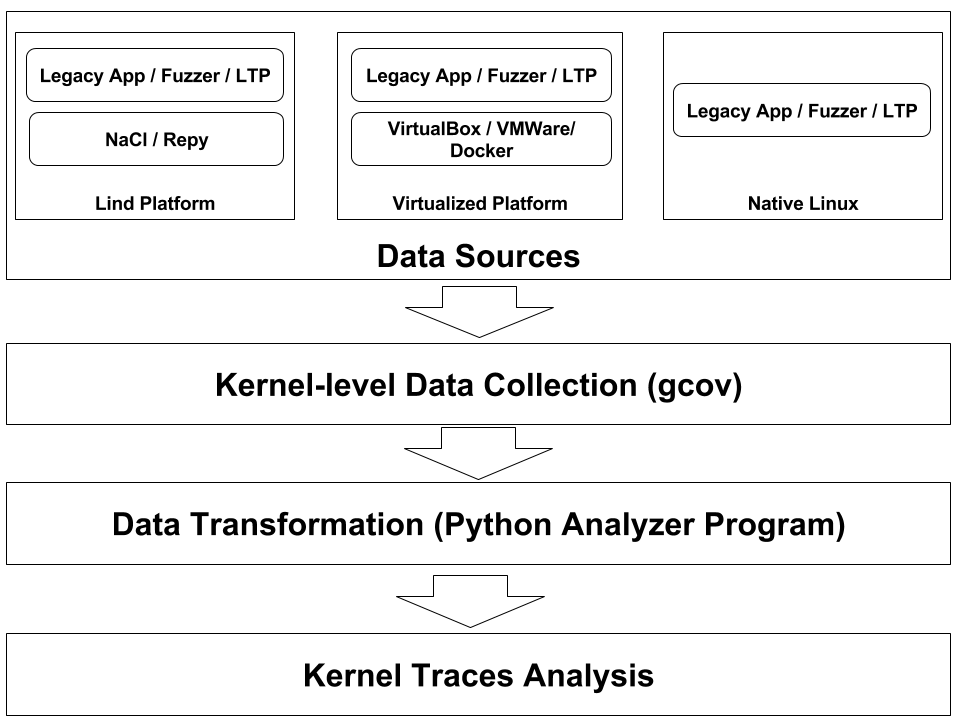
\includegraphics[width=1.0\columnwidth]{diagram/data_collection.png}
%\caption{Various activities performed to capture and analyze the kernel
% traces generated by legacy applications, system fuzzers, LTP, and CVE bug
% reports. The traces are collected using \texttt{gcov} and a Python-based
% program that transforms the gcov data to
% macrodata-level information of each traversed path for final data analysis.
%\cappos{I'm not sure what the point of this is...  Also, when are Docker
%and Lind used in gathering the metric data!?!}}
% %\loistransformed to what? And, how?
%
%\label{fig:datacollection}
%\end{figure}

%\yanyan{I feel this is a bit early to make this conclusion.}
%\lois{does the slight wording change answer your concern, Yanyan?}



%Although the total reachable paths coverage is not 100\% of the entire
%kernel code base,
%it is still very large and contains many bugs.
%However, because the commonly used kernel path coverage is much smaller
%than
%the total reachable path coverage, this is a positive indication that these
%relatively small areas can be considered safe.

%\begin{table}
%\centering
%\scriptsize
%\caption {Kernel Coverage}
%\begin{tabular}{|l|c|}
%  \hline
%  \textbf{Kernel Paths} & \textbf{Kernel Coverage (percentage)} \\
%  \hline \hline
%  Common Paths & 12.4\% \\
%  \hline
%  Total Reachable Paths & 32.2\% \\
%  \hline
%\end{tabular}
%\label{table:kernel_coverage}
%\end{table}

%\begin{figure}
%	\centering
%	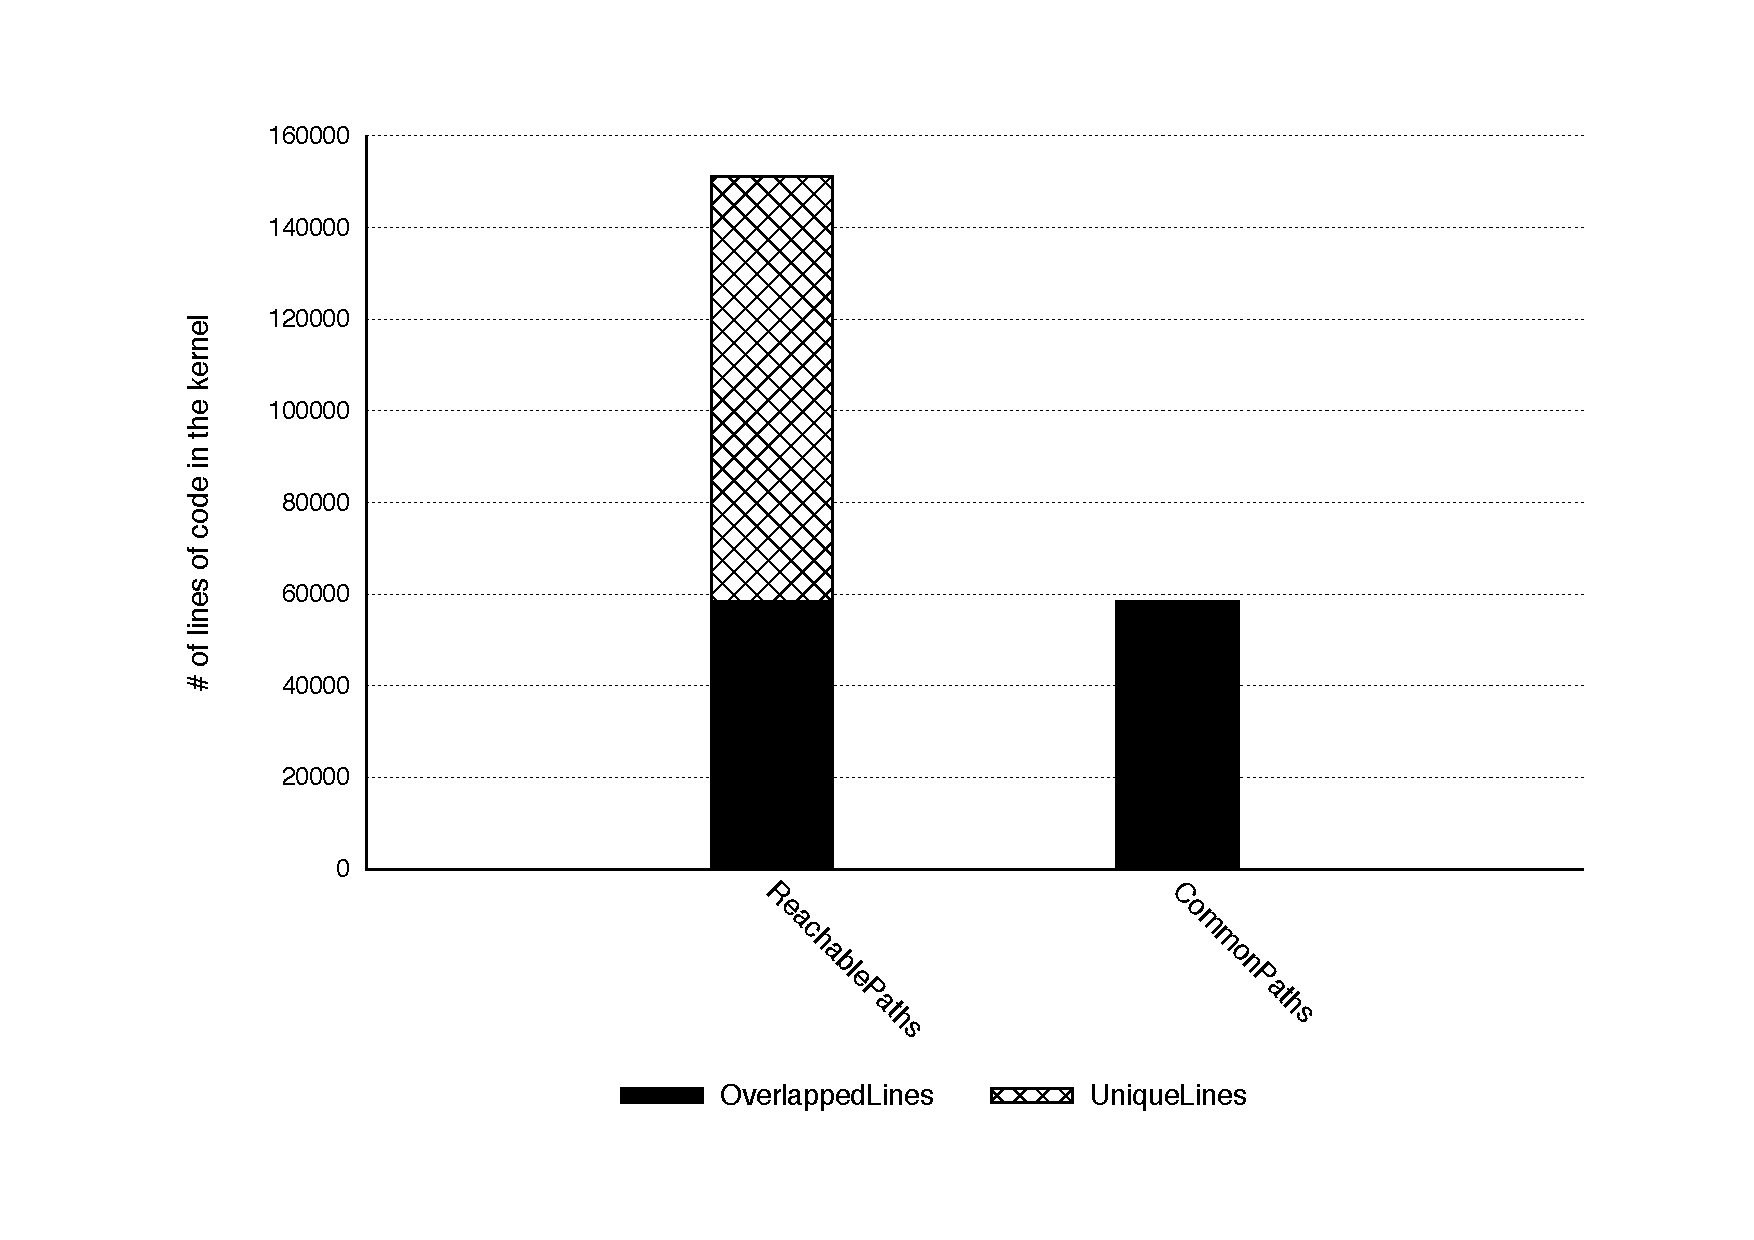
\includegraphics[width=1.0\columnwidth]{diagram/lind_oakland16_diagram_01.pdf}
%	\caption{Kernel Trace Comparison: Common paths as a subset of reachable paths}
%	\label{fig:subset}
%	\end{figure}
%
%	\begin{figure}
%	\centering
%	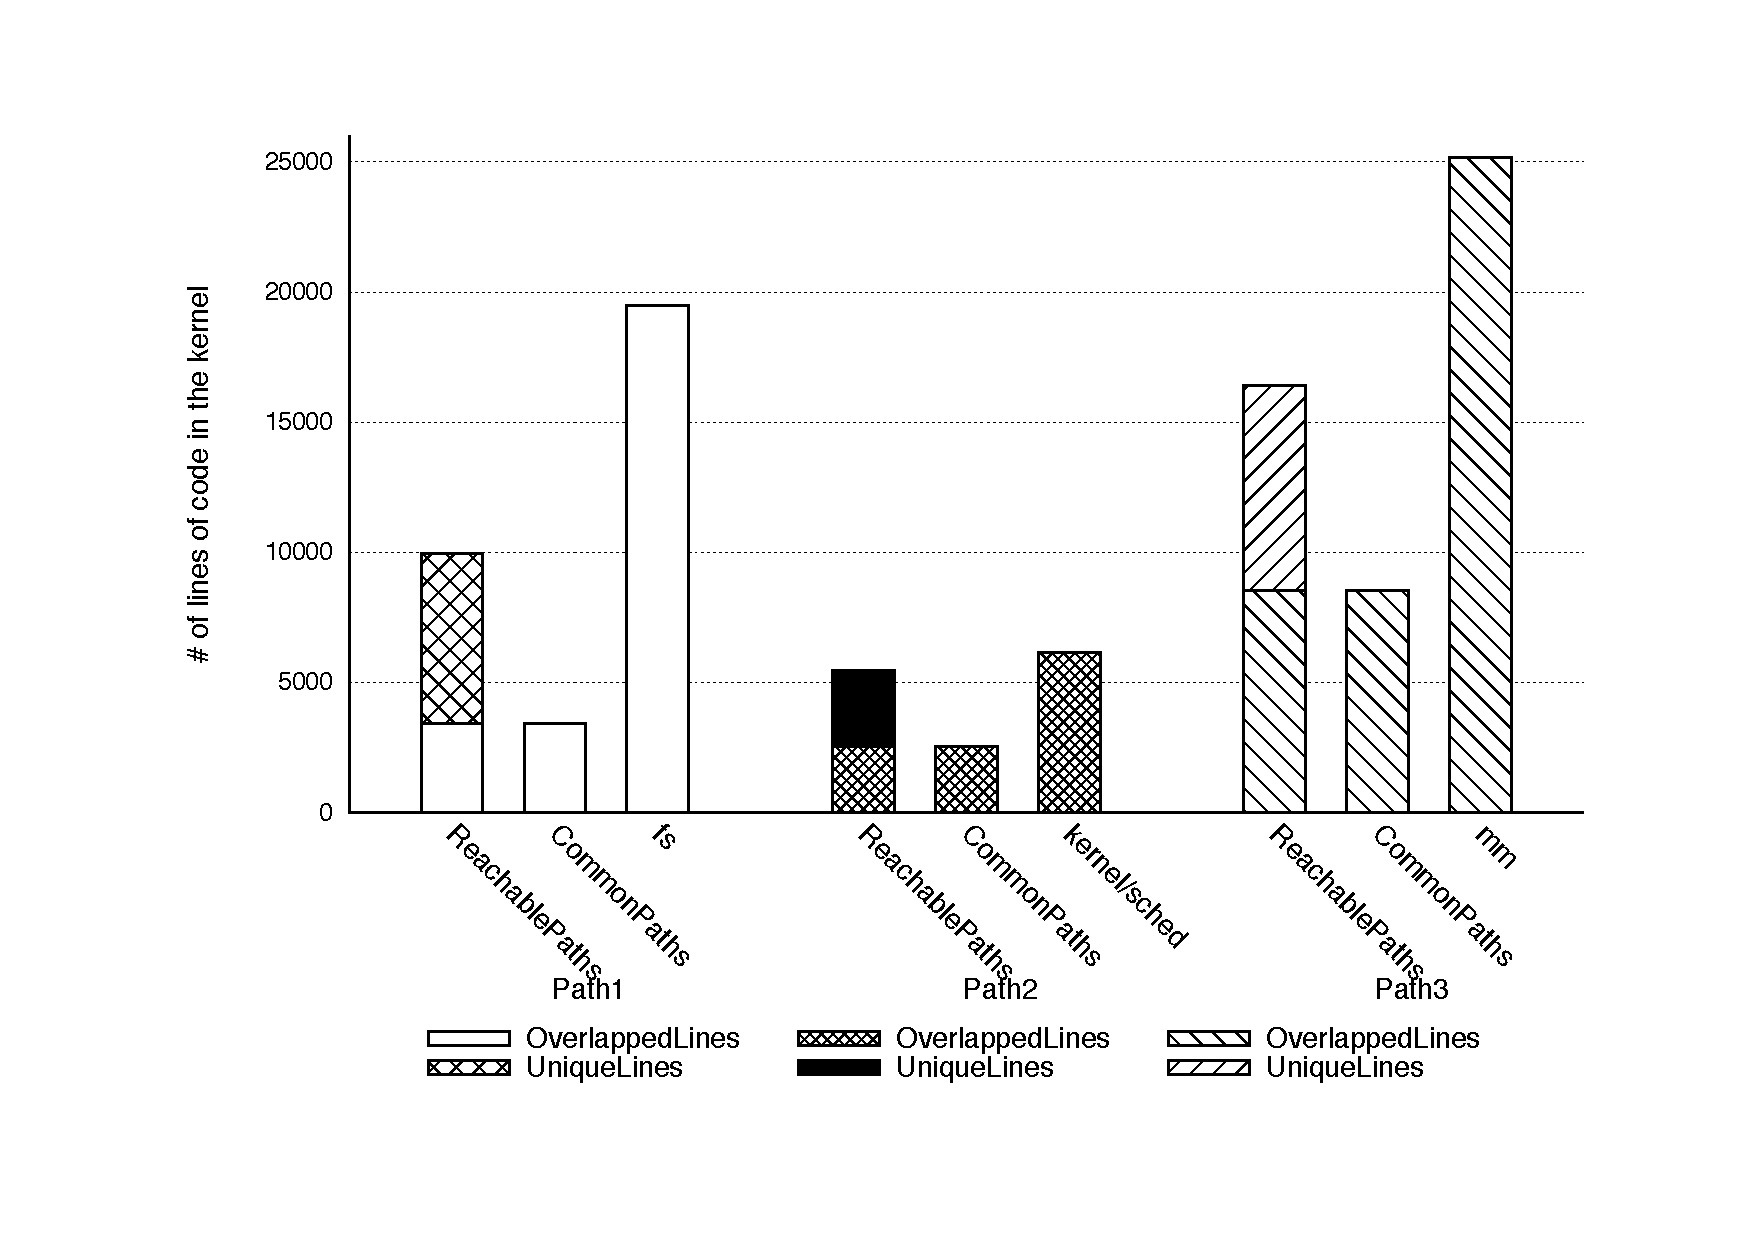
\includegraphics[width=1.0\columnwidth]{diagram/lind_oakland16_diagram_02.pdf}
%	\caption{Kernel Trace in Key Paths.  \cappos{I don't understand what 
%this is saying that isn't said before.}}
%	\label{fig:key_paths_trace}
%\end{figure}








%\begin{table*}[!ht]
%\scriptsize
%\centering
%
%\caption {Linux Kernel Bugs, and Vulnerabilities in Different Portions of
%the Kernel
%({\color{red}\ding{51}}: vulnerability in paths; \ding{55}: vulnerability
%not in paths) \cappos{This table will be TRed} }
%
%\begin{tabular}{|l|l|c|c|}\hline
%\multirow{2}{*}{\textbf{Vulnerability}} & \multirow{2}{*}{\textbf{Specific
%Type}} & \multicolumn{2}{c|}{\bf Portion of the Kernel} \\
%\cline{3-4}
%&  & \textbf{Total Reachable Paths} &  \textbf{Common Paths} \\ \hline
%
% CVE-2014-9529 & concurrency, race condition & {\color{red}\ding{51}} &
%\ding{55} \\
% CVE-2014-3631 & NULL pointer dereference & {\color{red}\ding{51}} &
%\ding{55} \\
% CVE-2012-6657 & network socket variable mischeck & {\color{red}\ding{51}}
%& \ding{55} \\
% CVE-2014-5207 & privilege escalation & \ding{55} & \ding{55} \\
% CVE-2014-5206 & privilege escalation & \ding{55} & \ding{55} \\
% CVE-2014-3153 & privilege escalation & \ding{55} & \ding{55} \\
% CVE-2014-2851 & privilege escalation & \ding{55} & \ding{55} \\
% CVE-2014-2706 & race condition, DoS & {\color{red}\ding{51}} & \ding{55}
%\\
% CVE-2014-0100 & race condition, DoS & {\color{red}\ding{51}} & \ding{55}
%\\
% CVE-2014-0049 & buffer overflow & \ding{55} & \ding{55} \\
% CVE-2012-6638 & DoS & {\color{red}\ding{51}} & \ding{55} \\
% CVE-2014-0038 & privilege escalation & \ding{55} & \ding{55} \\
% CVE-2013-6368 & privilege escalation & \ding{55} & \ding{55} \\
% CVE-2013-4587 & index error, privilege escalation & \ding{55} & \ding{55}
%\\
% CVE-2013-4563 & size/boundary check, DoS & {\color{red}\ding{51}} &
%\ding{55} \\
% CVE-2013-4348 & value validation error & \ding{55} & \ding{55} \\
% CVE-2013-4300 & privilege escalation & {\color{red}\ding{51}} & \ding{55}
%\\
% CVE-2013-1943 & privilege escalation & \ding{55} & \ding{55} \\
% CVE-2013-2094 & privilege escalation & {\color{red}\ding{51}} & \ding{55}
%\\
% CVE-2013-3301 & NULL pointer dereference, DoS & {\color{red}\ding{51}} &
%\ding{55} \\
% CVE-2013-1858 & privilege escalation & {\color{red}\ding{51}} & \ding{55}
%\\
% CVE-2013-1797 & use-after-free & {\color{red}\ding{51}} & \ding{55} \\
% CVE-2013-1763 & privilege escalation, index error & \ding{55} & \ding{55}
%\\
% CVE-2013-0310 & NULL pointer dereference & \ding{55} & \ding{55} \\
% CVE-2012-2136 & heap-based buffer overflow & \ding{55} & \ding{55} \\
% CVE-2012-2100 & lack of sanity check  & \ding{55} & \ding{55} \\
% CVE-2012-0028 & privilege escalation & {\color{red}\ding{51}} & \ding{55}
%\\
% CVE-2011-2517 & privilege escalation, buffer overflow &
%{\color{red}\ding{51}} & \ding{55} \\
% CVE-2012-2123 & privilege escalation  & {\color{red}\ding{51}} & \ding{55}
%\\
% CVE-2012-1146 & NULL pointer dereference  & \ding{55} & \ding{55} \\
% CVE-2012-0207 & divide-by-zero error and panic & \ding{55} & \ding{55} \\
% CVE-2011-2525 & NULL pointer dereference  & {\color{red}\ding{51}} &
%\ding{55} \\
% CVE-2011-1076 & NULL pointer dereference  & {\color{red}\ding{51}} &
%\ding{55} \\
% CVE-2011-2184 & NULL pointer dereference, none initialization & \ding{55}
%& \ding{55} \\
% CVE-2010-2478 & integer overflow & {\color{red}\ding{51}} & \ding{55} \\
% CVE-2010-2960 & NULL pointer dereference  & \ding{55} & \ding{55} \\
% CVE-2010-2492 & privilege escalation, buffer overflow & \ding{55} &
%\ding{55} \\
% CVE-2010-2240 & stack overflow & {\color{red}\ding{51}} &
%{\color{red}\ding{51}}\\
% CVE-2010-1188 & use-after-free & \ding{55} & \ding{55} \\
% CVE-2010-0437 & NULL pointer dereference  & {\color{red}\ding{51}} &
%\ding{55} \\ \hline
% \multicolumn{2}{|c|}{\bf Percentage contains bugs} & {\bf $50\%$} & {\bf
%$2.5\%$} \\ \hline
%\end{tabular}
%\label{table:vulnerabilities_commonly_used_kernel_paths}
%\end{table*}

%We studied bugs from the large-scale NVD database which includes representative bugs for all categories,
%and conducted experiments with ones with the highest vulnerability severity scores. This makes it a fair collection of available bugs sample
%to ensure the sample was not biased and it would be a normal distribution of bugs in the Linux kernel.
%\lois{Why does thismethod, which seems less than random, prove it is not biased?}


%Our hypothesis and findings provide insights and guidelines for new designs of secure systems, which will be discussed in the next section.
%\cappos{Is this statistically significant?}
%\yiwen{I added something to explain our bug sample dataset. More knowledge of statistics may be required. I will think about it more.}







\cappos{This will be trimmed...}
\subsection{Risk Metrics for Identifying Kernel Flaws}
\cappos{This section really doesn't tell me why these can't be used.  If you
say that this study uses a specific statistical method, why does this matter?
Why can't the Milk or Wine result for age be used? }

Even though there is no widely accepted method for
quantifying the safety (or risk) of privileged code, there have been a number of
attempts to measure flaws in both software and operating systems. In this section,
we briefly summarize a few of these approaches. Additional information on
past studies of potential flaws.

%\cappos{Is this really true?  No one has ever proposed a metric?  We do need to do a more detailed analysis of this.
%I would vote to remove this sentence regardless...} \lois{ I would agree its probably best just to get rid of the sentence.
%But I believe the goal here was to say that there is no widely accepted and used standard method.}


Other researchers have attempted to study the lifecycle of vulnerabilities�when they are
initiated and how long they last. Ozment and Schechter, who studied
vulnerabilities in the code base of an OpenBSD
operating system, determined that a significant extent (61%) of the reported
vulnerabilities were "foundational," meaning they were introduced prior to the
initial version studied. They also reported these vulnerabilities
have a median lifetime of at least 2.6 years.

These past methods can provide some insight on where bugs may lie in kernel and when
they may develop. However, most have relied on statistical methods, such as
negative binomial regression model~\cite{Bug-Location}. The metric we set out to
develop was to be based on empirical study of
the most critical bugs. This ad-hoc security metric can be used for
quantitative measurement and evaluation of the kernel bugs,
and other vulnerabilities at the level of lines of code by checking against
known kernel bugs.

We believe this metric will provide better understanding of kernel security.
As a result, a secure interface with an isolation mindset can be designed
to be exposed to the userspace.

%, they have limitations. Firstly, the metrics mentioned above are not specifically designed for studying bugs in OS kernels
%\cappos{Why does this matter?}

%Therefore, they do not take into account the way system calls are invoked by user applications.
%Moreover, these metrics can not provide information about the accurate location of the bugs within the kernel,
%which is important to our study.
%\cappos{Are you going to show that this is true?  Can you explain more about why these do not work?}
%\cappos{Do existing metrics work on a LOC level?  }

%Without any guidance as to what parts of the kernel are safe, past initiatives to protect the system through isolation,
%such as by building a sandbox or using library OSes, because they could not isolate user programs effectively.
%\cappos{What are you saying?} These methods can mitigate the problem, but any such system will still allow access to the kernel the same way as before.
%They simply move the attack surface from between the user space and the kernel, \yanyan{what's the purpose/consequence of this move?
%why is this move good or bad?} to between these new systems and the kernel, but the surface is not necessarily reduced.
%As a result, the proposed solutions do not make the systems more secure.

%Recognizing this limitation, we propose a novel security metric to
%\lois{does the metric itself tell us HOW to safely-reimplment? Or just tell us whether it needs this reimplementation?}

%\yanyan{I don't think the new metric alerts us tho. maybe say it provides
%as a guidance which parts are risky?} \cappos{end of text}


Other work has generated vulnerability
signatures~\cite{brumley2006towards}, which match all exploits
of a given flaw. Most of this work is based on a mix of static and
dynamic analysis, constraint solving and symbolic execution~\cite{chou2003static}.


\begin{figure}%[h]
\centering
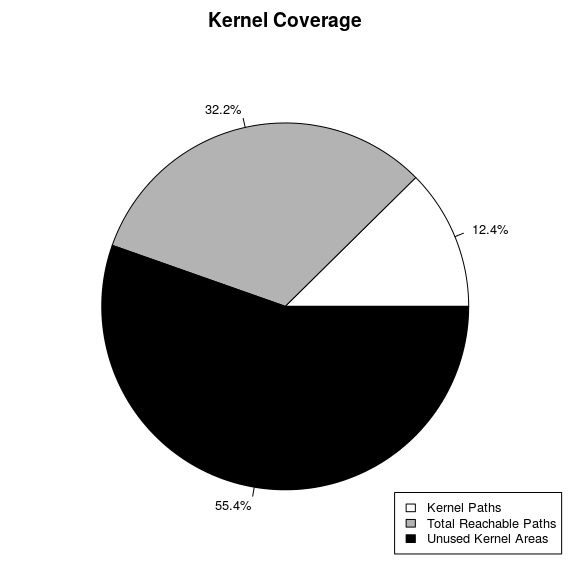
\includegraphics[width=1.0\columnwidth]{diagram/kernelcoverage.png}
\caption{Percentage of different kernel areas that were reached during
 LTP and Trinity system call fuzzing experiments.
 \yiwen{This figure will be replaced. I am working on a new one that will show 
 where different bugs are located.}}
\label{fig:coverage}
\end{figure}

